\chapter{Models and Methods}

The models presented in chapter~\ref{relevant-models} seem to work well in the context of adaptive systems. But could the performance be further improved by taking into account the timing information of students' answers (i.e. the response times or the breaks between practices)? As was discussed in chapter~\ref{spacing-effect}, the spacing effect is observable in environments where the students have no prior knowledge. We are interested primarily in domains where the prior knowledge varies widely between students.

\section{Models Based on Timing Information}

In this chapter we discuss several models which aim at modeling students' memory with the usage of timing information of answers. There are several several issues to consider beforehand:

\begin{itemize}
  \item Students have different skills and thus the rate of retention loss varies.
  \item The difficulty of items varies, some items are forgotten faster and some slower.
  \item The prior knowledge of each student is different. If the student already has the practiced item in their long term memory, the process of forgetting is much slower.
\end{itemize}

\subsection{PFA: The Extended Model}

One possibility how to incorporate timing information into the PFA model is by changing the memory activation in prediction. The times of previous attempts are passed to a \textit{time effect function} which may increase the probability of recall (see Equation~\ref{eq-pfa-standard-time-p}).

\begin{equation} \label{eq-pfa-standard-time-p}
  P(m) = \frac{1}{1 + e^{-(m + f(t))}}
\end{equation}

Since this is an extension of the standard PFA model, it is possible to integrate the estimation of prior knowledge as well as the probability of guessing into the model.

\subsection{PFA: The Alternative Model}

Another way of dealing with timing between attempts is by changing the decay factor $\xi$ of the model presented in chapter~\ref{pfa}. The model takes into account the order of questions, yet doesn't consider timing between student's practices of an item. This problem can be resolved by replacing the parameter $\xi$ with time effect functions.

\begin{equation} \label{eq-pfa-gong-time-s}
  s_{i,j} = \sum_{k=1}^{n-1} y_k \cdot f(t_k)
\end{equation}

\begin{equation} \label{eq-pfa-gong-time-f}
  f_{i,j} = \sum_{k=1}^{n-1} |y_k - 1| \cdot g(t_k)
\end{equation}

Equations~\ref{eq-pfa-gong-time-s},~\ref{eq-pfa-gong-time-f} show the incorporation of the time effect function $f$ and $g$ in the model. The parameter $t_k$ represents the number of seconds that passed between the $k$-th practice and the most recent one. The weight of successes and failures is thus dependent on the ages of the prior practices.

As was discussed in the chapter~\ref{pfa}, the problem arises with multiple-choice questions. Another difficulty is the choice of a time effect function that fits the data well. The function should theoretically represent the rate at witch the effect of learning decays with the passage of time.

\subsection{PFA: The Spacing Effect}

\todo{Better and more extensive explanation (experiments aren't quite finished yet).}

Time effect function is applied only if the student's answers were mostly incorrect (the student probably doesn't have the knowledge of the fact in their long-term memory).

\section{Fitting Parameters}

The goal of the fitting procedure is to find the optimal parameters that perform well on new samples (in our case predict the student's ability to answer a question correctly). In this chapter we describe some metrics commonly used for the evaluation of predictive performance (i.e. the fitness of parameters in the model) and the principal algorithms that are suitable for parameter estimation in our case.

\subsection{Metrics}

In our case we are not only interested in the correctness of student's answers, our aim is to predict the probability of correct answer as it may indicate how well the student knows the answer. The information of student's knowledge is crucial if we don't want the student to be demotivated by overly difficult or simple questions.

\begin{equation} \label{rmse}
  RMSE = \sqrt{\frac{\sum_{i=1}^n (x_i - y_i)^2}{n}}
\end{equation}

\begin{equation} \label{ll}
  LL = \sum_{i=1}^n y_i \log(x_i) + (1 - y_i) \log(1 - x_i)
\end{equation}

\subsection{Grid Search}

\begin{figure}[htbp]
  \centering
  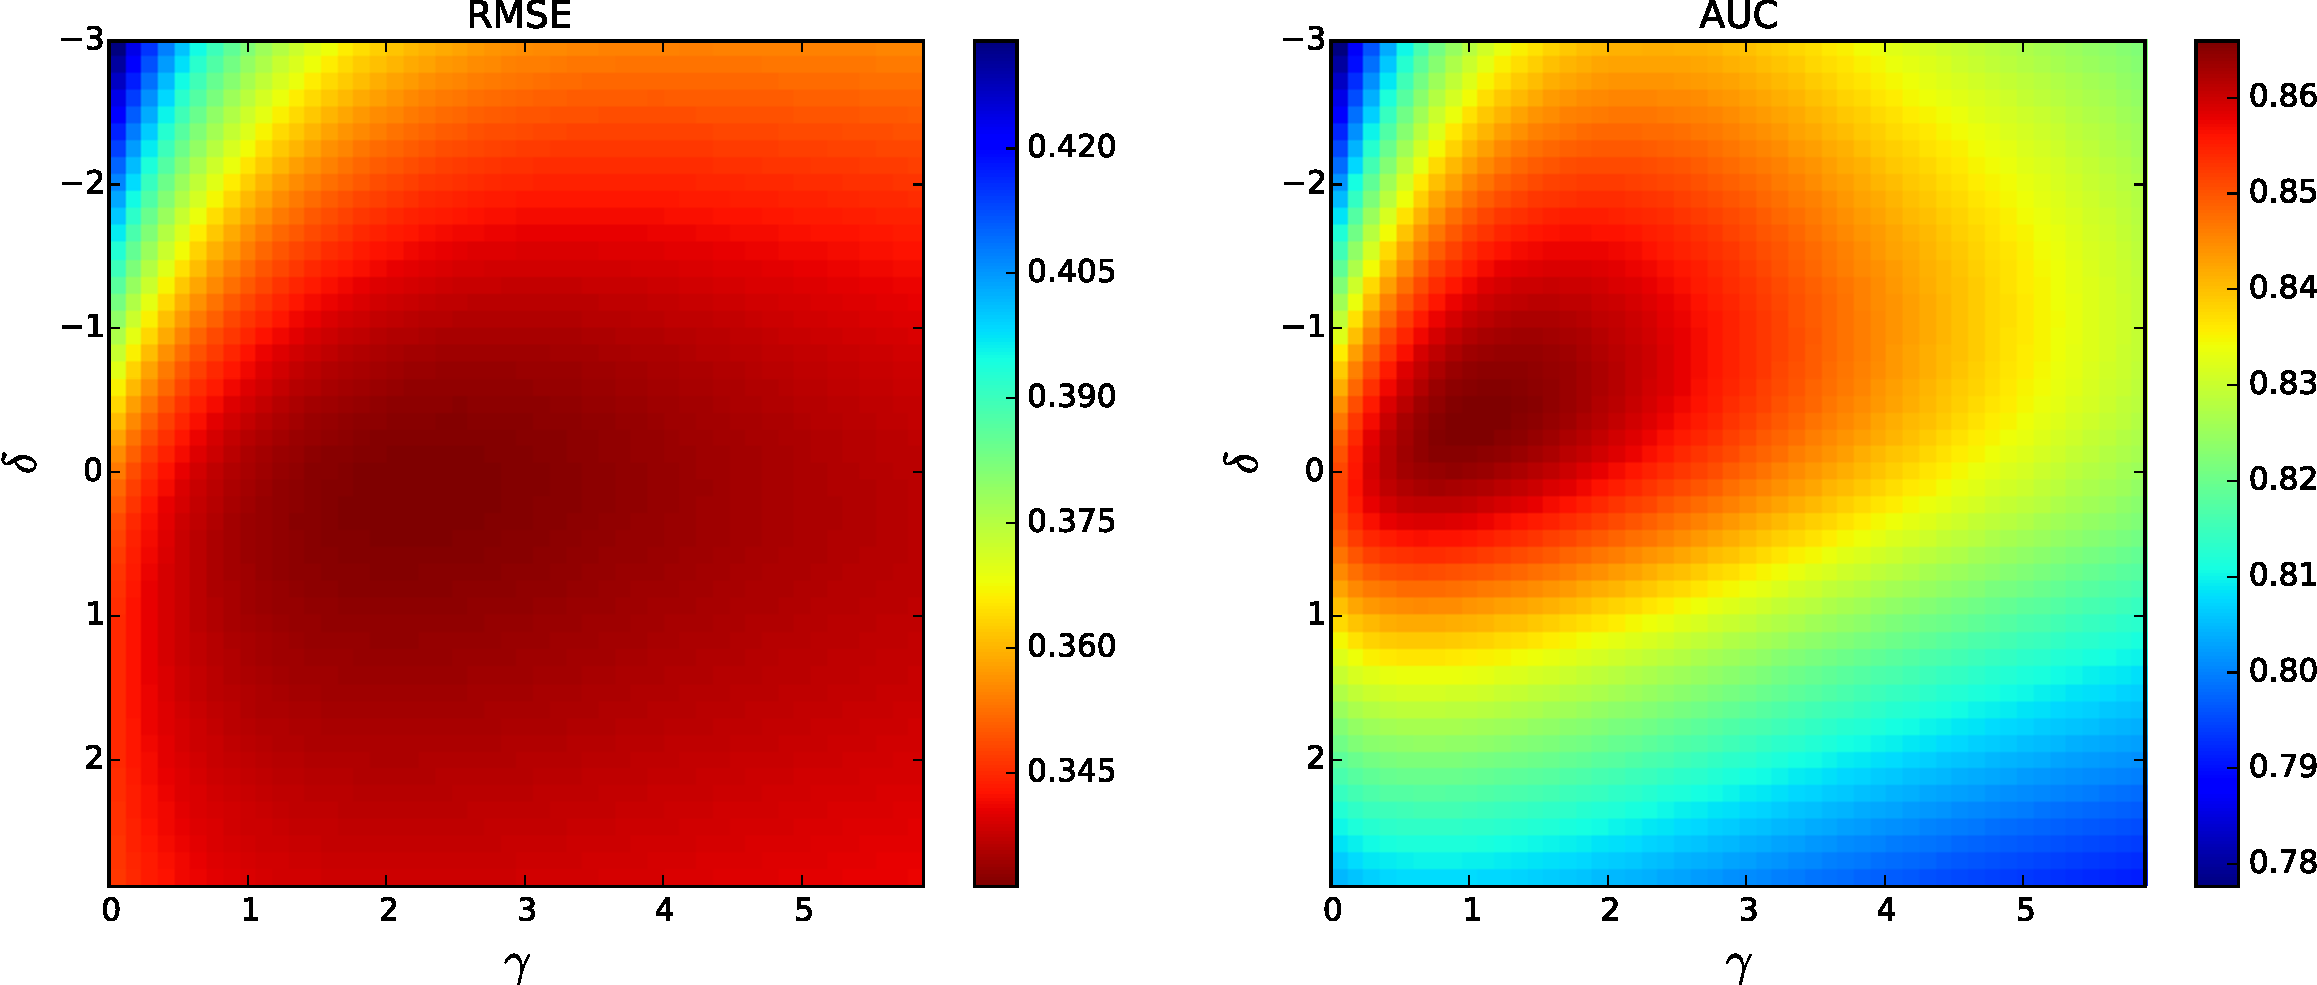
\includegraphics[width=\textwidth]{img/pfa-grid-search-rmse-auc}
  \caption{Result of the grid search performed on the PFAE model.}
  \label{fig-grid-search-rmse-auc}
\end{figure}

\subsection{Random Search}
